\chapter{Methods used for \acrshort{ci} Framework}
To overcome the problems discussed in Section \ref{current problem}, this thesis proposes a solution to automate the process of testing standalone modules
in Optislang. Since, the process is automated, the testing of modules needs to be done without the help of the \acrshort{gui}. To achieve this, a Python based 
framework is created to test the modules in an according manner. To run the framework, a \acrshort{ci} pipeline is created using GitHub Actions. The pipeline 
is triggered whenever a new commit is pushed to the repository. The pipeline runs the tests on the modules in a virtual machine and checks if the outputs are as expected. If the tests 
fail, the pipeline provides feedback to the developer about the failure. The developer can then look into the issue and resolve it. 

Many modern software engineering methods and practices are applied in this thesis. The following sections discuss these best practices and their implementation in the thesis. 
\section{DevOps}
\subsection{Introduction}
In former days, software development was divided into two separate phases: development and operations. The development team was responsible for writing the code and 
building the software, while the operations team was responsible for deploying and maintaining the software. If the software failed in production, the operations 
team would send the software back to the development team for fixing. This division of responsibilities often led to many issues
\begin{itemize}
    \item Developers needed to wait for the feedback from the operations team, which slowed down the development process.
    \item Developers passed the software to the operations team without knowing how it would perform in production, which led to many issues.
    \item Collaboration between the development and operations teams was limited, which made it difficult to resolve issues quickly and efficiently.
\end{itemize}

To overcome these challenges, DevOps was introduced. \textbf{DevOps} is a software development approach which encourages the collaboration between development(Dev) 
and operations(Ops) team \cite{10616918}. From this collaboration, the software development lifecycle is faster, more efficient and more reliable. These teams 
implement processes and tools to automate labour intensive, manual tasks which were slowing down the software development process. This also eliminates the 
need to depend on the other team for immediate feedback. 


\subsection{DevOps Lifecycle}
DevOps lifecycle is a set of phases, which brings in the development and operations group together to manage the entire software development lifecycle.
During each of the phases, different practices and tools are used to automate and streamline the software development process. Figure \ref{devops_lifecycle} shows 
the DevOps lifecycle. The development phase is depicted on the left side of the loop, whereas the operations phase is depicted on the right side of the loop. 
The loop represents the continuous nature of the DevOps lifecycle.
\begin{figure}[!ht]
    \centering
    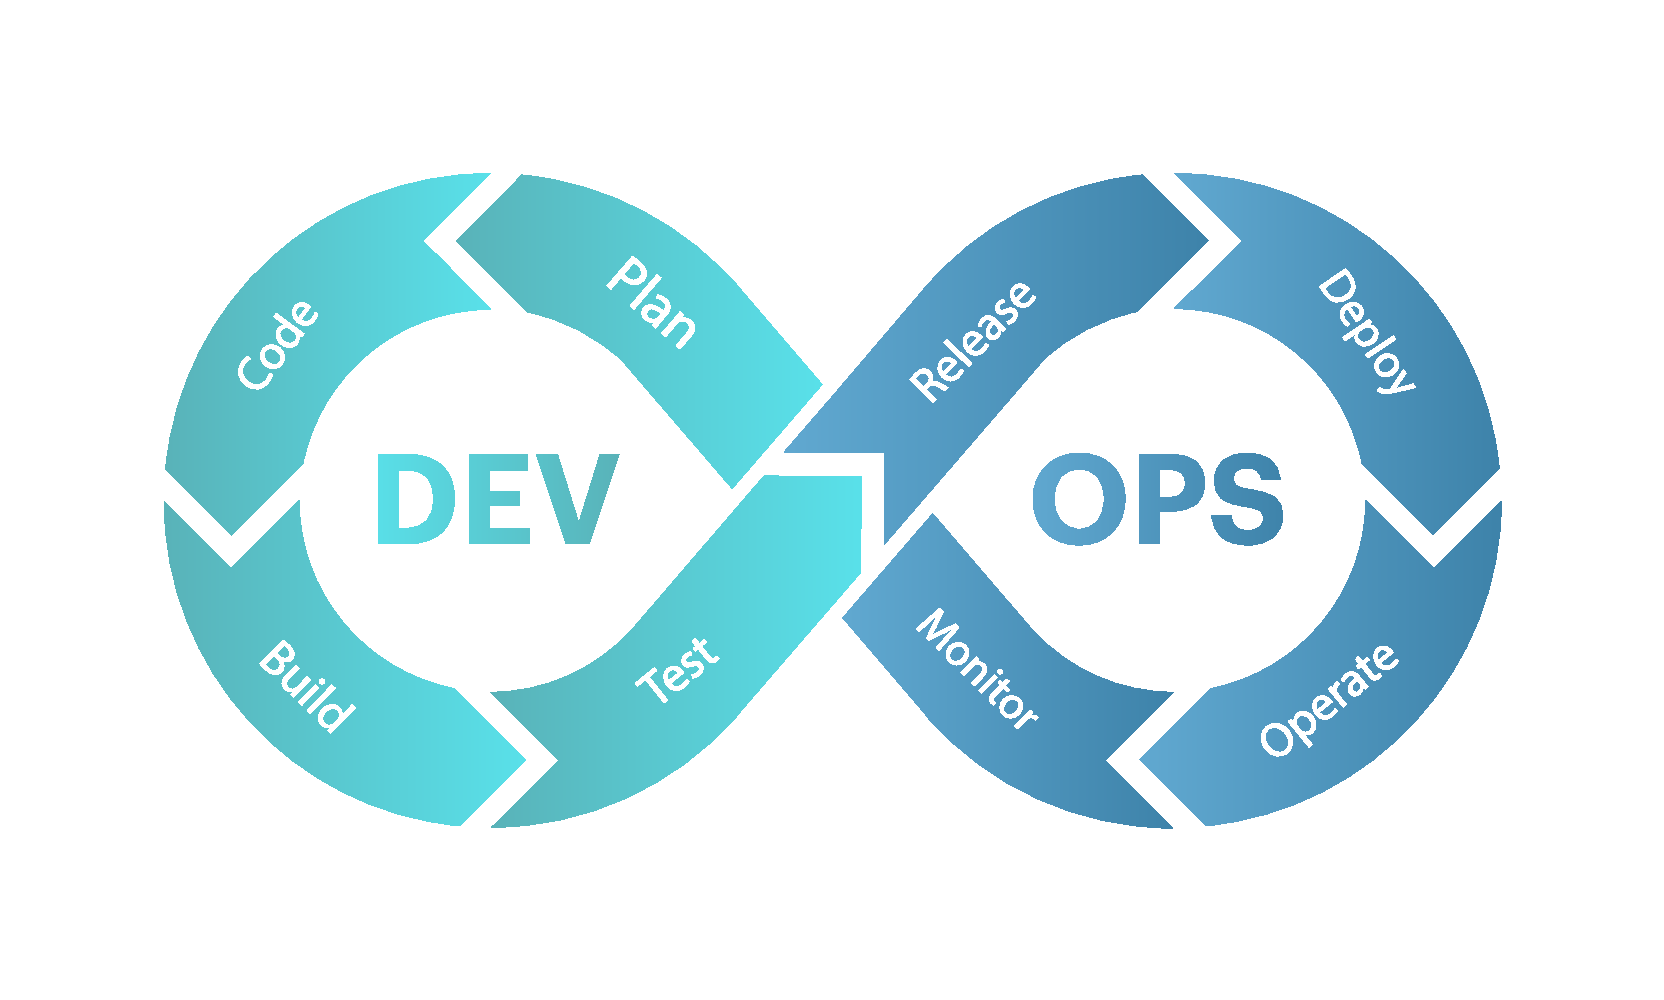
\includegraphics[width=0.7\textwidth]{Images/DevOps-Life-Cycle.pdf}
    \caption{DevOps Lifecycle \cite{devops_lifecycle}}
    \label{devops_lifecycle}
\end{figure}

The DevOps lifecycle consists of the following phases:
\begin{itemize}
    \item \textbf{Plan}:\newline
    The initial phase of any software development process is planning. During this stage, teams outline and prioritize the features to be developed. 
    This involves defining requirements, setting objectives, and creating a project roadmap.

    \item \textbf{Code}:\newline
    After the requirements are defined, developers start implementing the code. Developers must adhere to the coding standards, versioning and collaborating
    with other developers to ensure code quality.

    \item \textbf{Build}:\newline
    The build phase involves compiling the code and packaging the software. This phase ensures that the code is error-free and ready for deployment across 
    different environments.

    \item \textbf{Test}:\newline
    The testing phase involves running various automated tests to ensure that the software meets the requirements and is free of bugs. This phase includes 
    unit tests, integration tests, and system tests. This helps to identify and fix issues early in the development process.

    \item \textbf{Release}:\newline
    After the code has been tested and verified, it is released to the production environment. After verifying the code from bugs and errors, the code is 
    passed on the next phase.

    \item \textbf{Deploy}:\newline
    The code is automatically deployed to the production environment. This phase involves setting up the infrastructure, configuring the servers, and 
    deploying the software.

    \item \textbf{Operate}:\newline
    The operations team is responsible for verifying that the software is operating smoothly in the production environment.
    
    \item \textbf{Monitor}:\newline
    To verify if the software is running smoothly, the operations team monitors the software. This phase involves collecting and analyzing data to identify
    the health, performance, and security of the software. This data is used to identify and fix issues before they impact the end-users.
\end{itemize}

DevOps practices play a crucial role in the development of the automation process described in this thesis. By integrating \acrfull{ci} and \acrfull{cd} pipelines, 
efficiency and reliability while testing the modules is ensured. This helps us to improve productivity and reduce human error. According to \cite{8257807}, DevOps is not only helping to bridge
the gap between development and operations teams, but also helping to improve the quality of the software.
The DevOps approach allows for seamless collaboration between development and operations teams, 
ensuring that the testing framework and the modules it tests are consistently maintained and updated. This integration of DevOps practices not only enhances the quality of the software but also 
accelerates the development lifecycle, enabling faster delivery of new updates and features.\newline

In summary, the application of DevOps in this thesis demonstrates how modern software engineering practices can be applied to automate and streamline the testing process, leading to more robust,
efficient and reliable software solutions.

\section{\acrlong{ci}}
    \acrfull{ci} is the practice in software development where developers frequently commit their code changes to a shared repository. A \acrshort{ci} pipeline 
    can be applied to automate and streamline the testing process, leading to more robust, efficient and reliable software solutions \cite{8421965}.

    For the \acrshort{ci} pipeline to work, usually the code changes are stored in a version control system which can be collaborated by multiple developers.
    Examples of such version control systems are Bitbucket, GitLab and GitHub. A crucial practice of \acrshort{ci} is to commit the code changes to the repository 
    frequently \cite{6802994}. By implementing this practice, the codebase is always up-to-date and the developers can easily identify and fix issues early in 
    the development process. The main task of a \acrshort{ci} pipeline to inform the team whether the changes made to the codebase are correct or not. There are 
    several tools which provide this functionality. Some of the popular tools are Jenkins, Travis CI, Circle CI, GitHub Actions. 

    Issues can arise while configuring the \acrshort{ci} pipeline. For example, the \acrshort{ci} pipeline can fail due to 
    incorrect configuration, or the changes made to the codebase can impact negatively to the end user. To overcome these issues, modern \acrshort{ci} pipelines are 
    equipped with features like logging, alerts, metrics, and notifications.

    In this thesis, GitHub is used as the primary platform for storing the files and GitHub Actions is used to implement a \acrshort{ci} pipeline. After the code 
    changes are committed, the \acrshort{ci} pipeline is triggered automatically. A detailed implementation of the \acrshort{ci} pipeline is discussed in 
    Chapter \ref{ci_pipeline}. 

\section{Version Control Strategies} \label{version_control}
To track changes in the codebase, version control is used. It acts as a safety net for the developers, allowing them to revert to the previous version of the 
codebase if something goes wrong. Git, Mercurial and many other distributed version control systems provides the same functionality. In this thesis, 
Git\footnote{\url{https://git-scm.com/URL}} is used as the primary version control system. This method of tracking is setup locally. To collaborate with other 
developers, the codebase needs to be pushed  to a remote repository. In our organization, GitHub is used as the main source for hosting the codebase. By hosting a remote
repository, developers can collaborate with each other, track changes, and manage the codebase effectively. Version control is considered to be an important
practice in DevOps, as they reduce the development time of a product and increase the quality of the software by frequent deployment.

While working on a feature, or a bug fix, developers tend to create a new branch in the repository, so that the main branch is not affected. There are two main 
branching strategies : long-lived branches and short-lived branches. 
\subsection{GitHub Flow}
This branching strategy is a simplified version of the Git Flow. It is a lightweight, branch-based workflow that is designed around deploying code to production. 
It uses the concepts of branches and pull requests, which is ideal for working in teams and frequent deployments.
%! Please update with the new image
%# Update the figure with feature instead of change in branches
\begin{figure}[!ht]
    \centering
    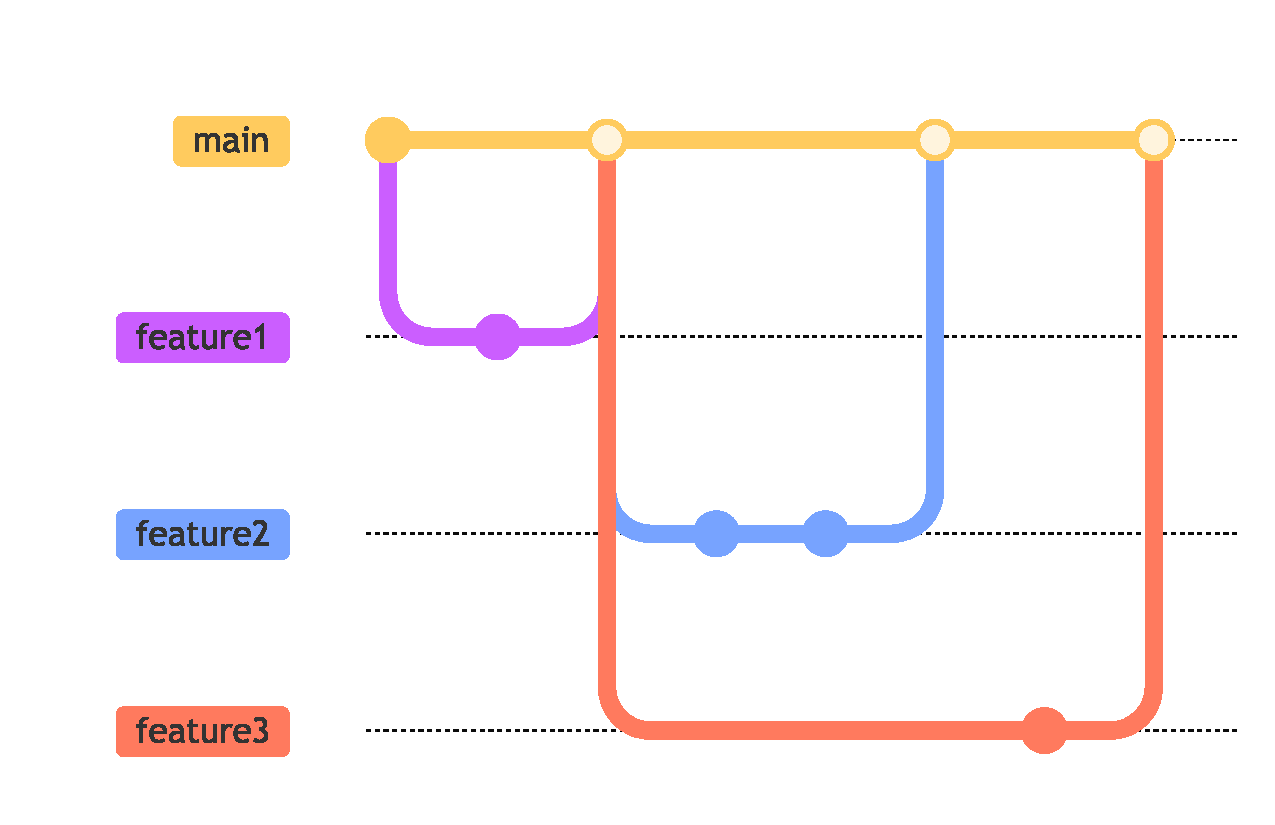
\includegraphics[width=0.7\textwidth]{Images/github_flow.pdf}
    \caption{Example of GitHub Flow}
    \label{github_flow}
\end{figure} 

\begin{itemize}
    \item \textbf{Main Branch}:\newline
    The main branch is the default branch in the repository. This branch is always deployable and contains the latest stable version of the code.

    \item \textbf{Feature Branch}:\newline
    When a new feature is to be implemented, a new branch is created from the main branch. This is practiced to avoid conflicts with the code in the main branch. 
    The developer works on the feature branch until the feature is completed. After the feature is completed, reviewed and tested, the branch is merged back to 
    the main branch. In the figure \ref{github_flow}, \texttt{feature1}, \texttt{feature2} and \texttt{feature3} are the feature branches.
\end{itemize}

GitHub Flow is simple to learn and implement and provides faster feedback to developers. 

\subsection{Git Flow}
Git Flow is a more complex branching model compared to GitHub Flow. It is a branching model that helps to manage the codebase in a more organized manner for
managing large projects with scheduled releases. It uses two long lived branches, master and develop, along with several short-lived branches.
%! Change the image here for the release branch
\begin{figure}[!ht]
    \centering
    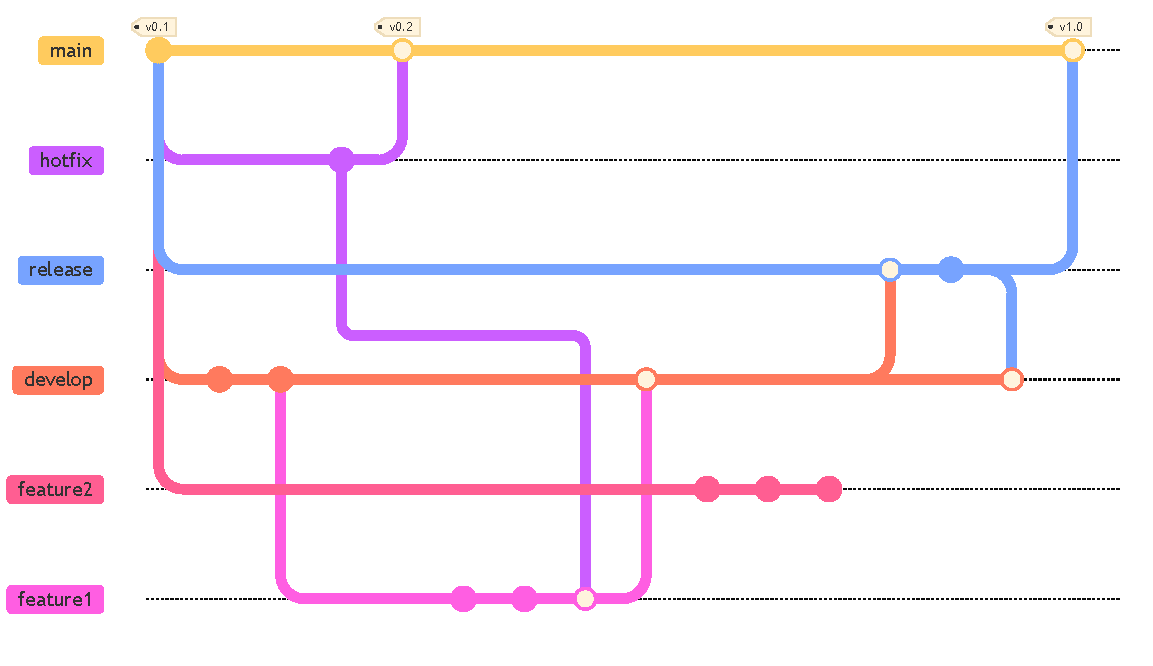
\includegraphics[width=0.9\textwidth]{Images/git_flow.pdf}
    \caption{Example of Git Flow}
    \label{git_flow}
\end{figure}
 \begin{itemize}
    \item \textbf{Main Branch}:\newline
    Main branch serves the same purpose as the main branch in GitHub Flow. It contains production ready code that can be released. Here, in figure \ref{git_flow},
    the main branch commits are tagged with their respective version numbers.

    \item \textbf{Develop Branch}:\newline
    This branch is created at the start of a project and contains pre-production code. This branch is maintained throughout the project and is used to merge 
    feature branches. The develop branch is merged to the release branch when the code is ready for release.

    \item \textbf{Feature Branch}:\newline
    This branch has the same responsibility as the feature branch in GitHub Flow. After the feature is implemented, the branch is merged with the develop branch.
 
    \item \textbf{Release Branch}:\newline
    This branch contains the code that is ready for release. It is created from the develop branch and is merged back to the main branch after the release.

    \item \textbf{Hotfix Branch}:\newline
    This branch is used to quickly address critical bugs in the production code. It is created from the main branch.
\end{itemize}

Git Flow is a more complex branching model compared to GitHub Flow. It is suitable for large projects with scheduled releases. It provides a more organized 
approach to managing the codebase and ensures that the code is stable and reliable before it is released to production. Due to the creation of several branches, 
developers can work parallel on different features without affecting the main branch.

\section{Code Quality}
Code quality is a critical aspect of software development that directly impacts the maintainability, reliability, and performance of the software. High-quality 
code is easier to understand, test, and modify, which is essential for the long-term success of any software project \cite{6862882}. In the context of this thesis, ensuring 
code quality is particularly important for several reasons:

\begin{itemize}
    \item \textbf{Maintainability}:\newline 
    High-quality code is well-structured and well-documented, making it easier for developers to understand and maintain. \acrshort{ci}/\acrshort{cd} pipelines 
    ensures the code quality is maintained throughout the development process, which is essential for the long-term success of the software. 
    \item \textbf{Reliability}:\newline 
    Code quality directly affects the reliability of the software. Well-written code is less prone to bugs and errors, which reduces the likelihood of failures 
    during the testing and deployment phases. This is particularly important in a DevOps environment, where the goal is to deliver reliable software quickly 
    and efficiently.
    \item \textbf{Efficiency}:\newline 
    High-quality code is optimized for performance, which can lead to faster execution times and more efficient use of resources. This is important for the 
    automation processes described in this thesis, as it ensures that the testing and deployment pipelines run smoothly and efficiently.
    \item \textbf{Collaboration}:\newline 
    In a collaborative environment, such as GitHub, high-quality code is essential for effective teamwork. Clear, well-documented code allows multiple contributors 
    to work on the same project without confusion or conflicts, which is a key aspect of successful \acrshort{ci} practices.
\end{itemize}

In summary, maintaining high code quality is essential for the success of the automation processes and the overall framework described in this thesis. It 
ensures that the software is maintainable, reliable, efficient, and conducive to collaboration, all of which are critical for achieving the goals of \acrlong{ci} 
and \acrlong{cd}.

\section{Frameworks}
\subsection{What is a Framework?}
A framework is a pre-built structure that provides a foundation for developing applications \cite{framework}. It includes libraries, tools, and best practices that accelerate 
the development process. Frameworks serve as templates that can be customized to meet project requirements. They allow developers to work on the core, i.e,
the application of logic, rather than worrying about the underlying structure. Many frameworks are open-source and are easily available. Developers can also
contribute to the framework by adding new features or fixing bugs.

It is crucial to first understand the project requirements and determine which programming language and corresponding framework best suit those needs. 
Each framework is designed for a specific purpose and offers unique features. Having a fundamental understanding of the chosen programming language is 
essential for effectively working with the framework. Popular frameworks used today include Django, Flask, Angular, React, PyTorch, TensorFlow, and more. 
These frameworks empower developers to create robust and feature-rich applications.

\subsection{Why is a Framework used?}
Developing code from scratch can be a tedious and error-prone task. Clean, well-tested, and bug-free code is essential, but achieving this can be challenging.
Additionally, developers must adhere to coding standards and best practices to ensure code quality. Therefore, using frameworks that meet the requirements is
a better choice. Frameworks simplify the development process, reduce errors and provide a general template that can be customized as needed. They also make it
easier for others to understand your code, as they are likely familiar with the frameworks used. Frameworks offer several advantages, including:
\begin{itemize}
    \item Simplified testing and debugging of code.
    \item Clean and understandable code.
    \item Reduced code redundancy within the project.
    \item Decreased project time and cost.
    \item Modifiable and extendable features and functionalities provided by the framework.
\end{itemize}

\subsection{Libraries vs Frameworks}It is a common misconception that libraries and frameworks are the same. But they serve different purposes and have distinct characteristics.
\subsubsection{Libraries:}
\begin{itemize}
    \item A library is a collection of pre-written code that developers can use to optimize tasks.
    \item It provides specific functionality that can be called upon when needed.
    \item Developers have control over the flow of the application and decide when to use the library.
    \item Some of the popular libraries include NumPy, Pandas, Matplotlib, and more.\newline
\end{itemize}


\subsubsection{Frameworks:}
\begin{itemize}
    \item A framework is a pre-built structure that provides a foundation for developing applications.
    \item It dictates the architecture and flow of the application.
    \item Developers must adhere to the structure and guidelines set by the framework.
    \item Examples of popular frameworks include Django, Flask, Angular, React, and more. \newline
\end{itemize}